\hypertarget{bintree_8c}{
\section{lib/bintree.c File Reference}
\label{bintree_8c}\index{lib/bintree.c@{lib/bintree.c}}
}
Binary tree implementation. 

{\tt \#include \char`\"{}arrow.h\char`\"{}}\par


Include dependency graph for bintree.c:\nopagebreak
\begin{figure}[H]
\begin{center}
\leavevmode
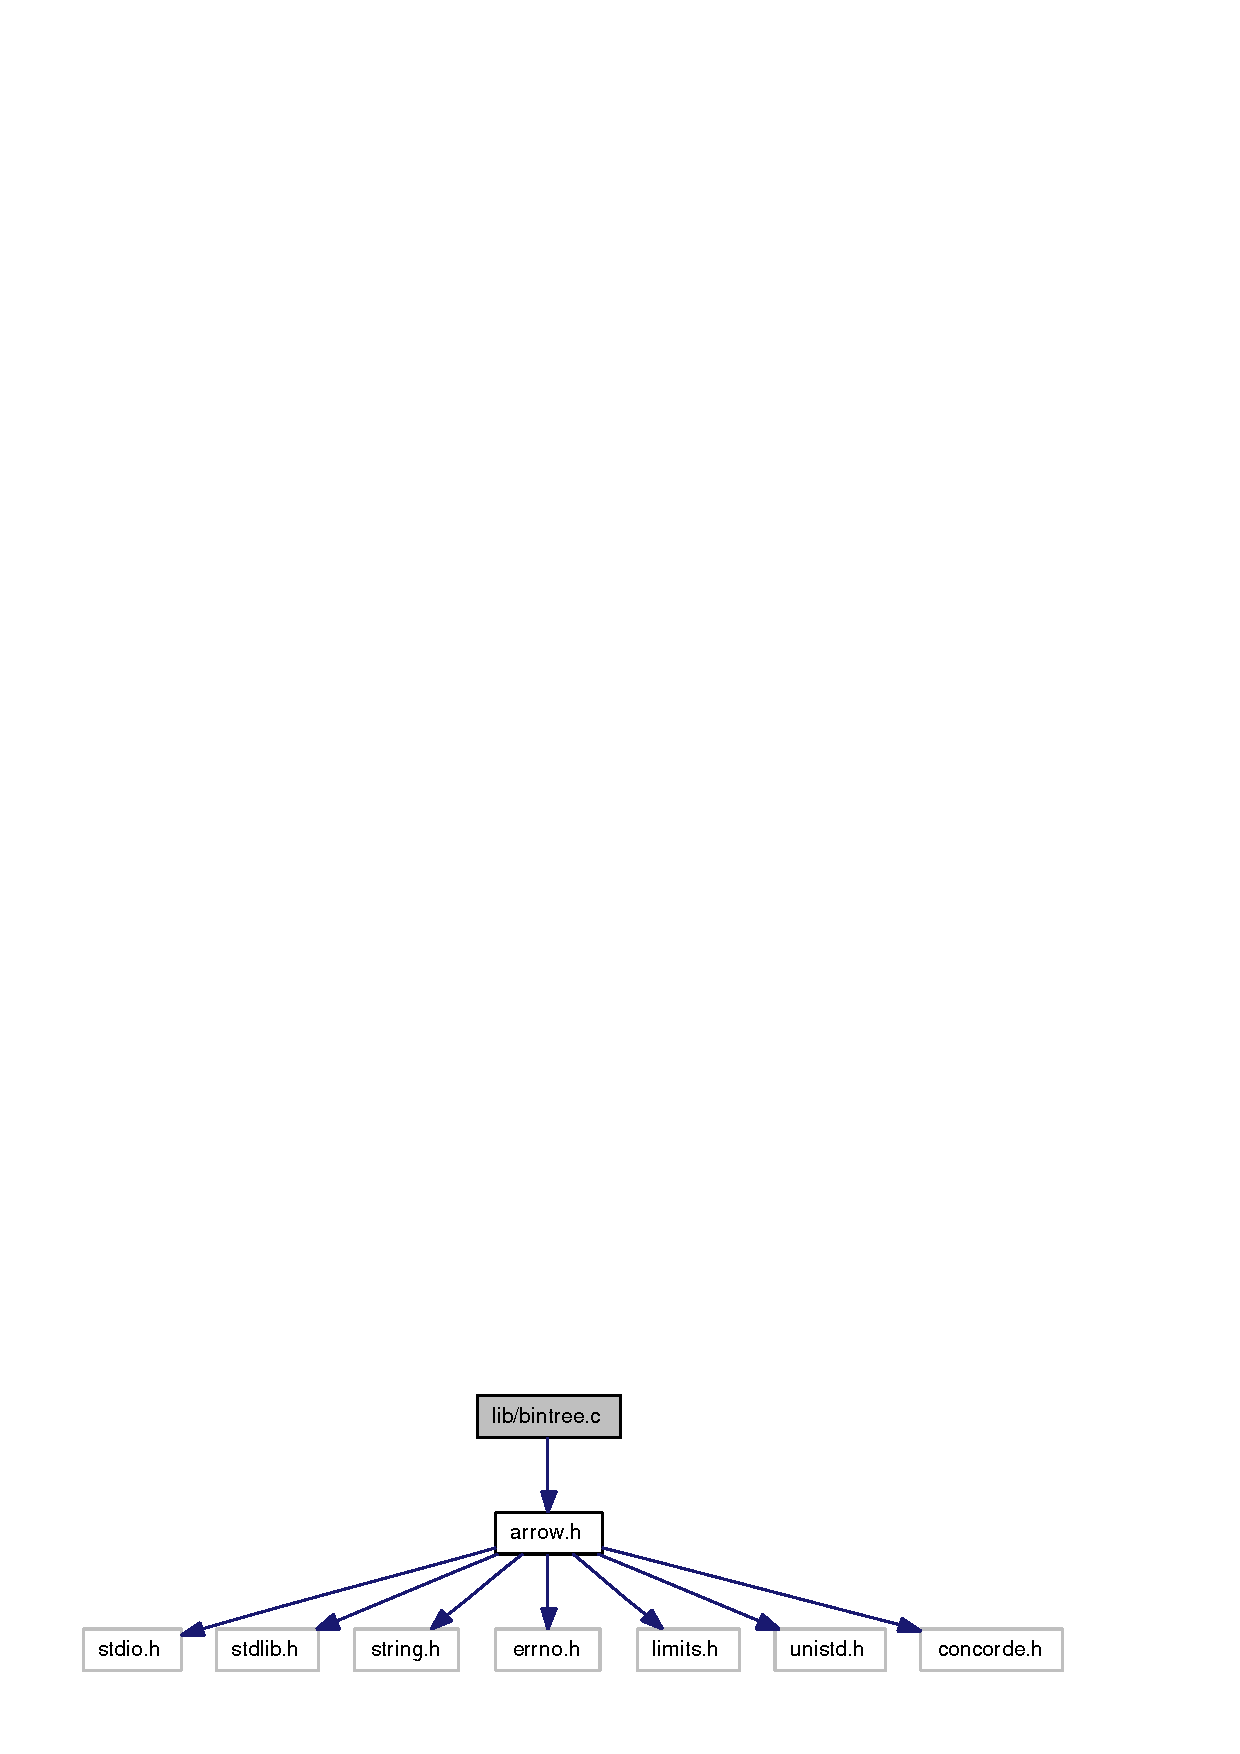
\includegraphics[width=257pt]{bintree_8c__incl}
\end{center}
\end{figure}
\subsection*{Functions}
\begin{CompactItemize}
\item 
int \hyperlink{bintree_8c_c252d0df6e75c9b8abe610c6e54fb9bc}{construct\_\-node} (\hyperlink{structarrow__bintree__node}{arrow\_\-bintree\_\-node} $\ast$$\ast$node, int value)
\begin{CompactList}\small\item\em Constructs a new arrow\_\-tree\_\-node structure with the given value. \item\end{CompactList}\item 
void \hyperlink{bintree_8c_5ecaa4df2e1066b8f541c223f4d19972}{destruct\_\-node} (\hyperlink{structarrow__bintree__node}{arrow\_\-bintree\_\-node} $\ast$node)
\begin{CompactList}\small\item\em Frees the memory of the given node and its child nodes. \item\end{CompactList}\item 
int \hyperlink{bintree_8c_363d994a11c0d61edb28f7ae03f1a6ac}{insert\_\-at} (\hyperlink{structarrow__bintree}{arrow\_\-bintree} $\ast$tree, \hyperlink{structarrow__bintree__node}{arrow\_\-bintree\_\-node} $\ast$node, int value)
\begin{CompactList}\small\item\em Inserts a given value into the tree at the given node, or one of its child nodes. \item\end{CompactList}\item 
void \hyperlink{bintree_8c_03a29b6ce9afff1e3a770b0af5f9b573}{fill\_\-array} (\hyperlink{structarrow__bintree__node}{arrow\_\-bintree\_\-node} $\ast$node, int $\ast$$\ast$array, int $\ast$pos)
\begin{CompactList}\small\item\em Recursive helper function to fill an array in nondecreasing order. \item\end{CompactList}\item 
void \hyperlink{bintree_8c_b28bc6559b228f0aa65cc671f67b9a09}{arrow\_\-bintree\_\-init} (\hyperlink{structarrow__bintree}{arrow\_\-bintree} $\ast$tree)
\begin{CompactList}\small\item\em Initializes the binary tree data structure. \item\end{CompactList}\item 
void \hyperlink{bintree_8c_ca9875422bf132eb9f5a4a2d10053207}{arrow\_\-bintree\_\-destruct} (\hyperlink{structarrow__bintree}{arrow\_\-bintree} $\ast$tree)
\begin{CompactList}\small\item\em Destructs a binary tree data structure. \item\end{CompactList}\item 
int \hyperlink{bintree_8c_75b4ee03b9667bd0e13e6cc71043e0a9}{arrow\_\-bintree\_\-insert} (\hyperlink{structarrow__bintree}{arrow\_\-bintree} $\ast$tree, int value)
\begin{CompactList}\small\item\em Inserts a value into the binary tree. \item\end{CompactList}\item 
int \hyperlink{bintree_8c_37fe2e7fbd64399611ba819ccfd5d4a2}{arrow\_\-bintree\_\-to\_\-array} (\hyperlink{structarrow__bintree}{arrow\_\-bintree} $\ast$tree, int $\ast$$\ast$array)
\begin{CompactList}\small\item\em Initializes the binary tree data structure. \item\end{CompactList}\end{CompactItemize}


\subsection{Detailed Description}
Binary tree implementation. 

Methods for working with Arrow's binary tree data structure.

\begin{Desc}
\item[Author:]John LaRusic \end{Desc}


Definition in file \hyperlink{bintree_8c-source}{bintree.c}.

\subsection{Function Documentation}
\hypertarget{bintree_8c_ca9875422bf132eb9f5a4a2d10053207}{
\index{bintree.c@{bintree.c}!arrow\_\-bintree\_\-destruct@{arrow\_\-bintree\_\-destruct}}
\index{arrow\_\-bintree\_\-destruct@{arrow\_\-bintree\_\-destruct}!bintree.c@{bintree.c}}
\subsubsection{\setlength{\rightskip}{0pt plus 5cm}void arrow\_\-bintree\_\-destruct ({\bf arrow\_\-bintree} $\ast$ {\em tree})}}
\label{bintree_8c_ca9875422bf132eb9f5a4a2d10053207}


Destructs a binary tree data structure. 

\begin{Desc}
\item[Parameters:]
\begin{description}
\item[{\em tree}]\mbox{[}out\mbox{]} binary tree structure \end{description}
\end{Desc}


Definition at line 59 of file bintree.c.

References destruct\_\-node(), arrow\_\-bintree::root\_\-node, and arrow\_\-bintree::size.

Referenced by arrow\_\-problem\_\-info\_\-get().\hypertarget{bintree_8c_b28bc6559b228f0aa65cc671f67b9a09}{
\index{bintree.c@{bintree.c}!arrow\_\-bintree\_\-init@{arrow\_\-bintree\_\-init}}
\index{arrow\_\-bintree\_\-init@{arrow\_\-bintree\_\-init}!bintree.c@{bintree.c}}
\subsubsection{\setlength{\rightskip}{0pt plus 5cm}void arrow\_\-bintree\_\-init ({\bf arrow\_\-bintree} $\ast$ {\em tree})}}
\label{bintree_8c_b28bc6559b228f0aa65cc671f67b9a09}


Initializes the binary tree data structure. 

\begin{Desc}
\item[Parameters:]
\begin{description}
\item[{\em tree}]\mbox{[}out\mbox{]} binary tree structure \end{description}
\end{Desc}


Definition at line 52 of file bintree.c.

References arrow\_\-bintree::root\_\-node, and arrow\_\-bintree::size.

Referenced by arrow\_\-problem\_\-info\_\-get().\hypertarget{bintree_8c_75b4ee03b9667bd0e13e6cc71043e0a9}{
\index{bintree.c@{bintree.c}!arrow\_\-bintree\_\-insert@{arrow\_\-bintree\_\-insert}}
\index{arrow\_\-bintree\_\-insert@{arrow\_\-bintree\_\-insert}!bintree.c@{bintree.c}}
\subsubsection{\setlength{\rightskip}{0pt plus 5cm}int arrow\_\-bintree\_\-insert ({\bf arrow\_\-bintree} $\ast$ {\em tree}, \/  int {\em value})}}
\label{bintree_8c_75b4ee03b9667bd0e13e6cc71043e0a9}


Inserts a value into the binary tree. 

\begin{Desc}
\item[Parameters:]
\begin{description}
\item[{\em tree}]\mbox{[}out\mbox{]} binary tree structure \item[{\em value}]\mbox{[}in\mbox{]} value to insert into tree \end{description}
\end{Desc}


Definition at line 66 of file bintree.c.

References construct\_\-node(), insert\_\-at(), arrow\_\-bintree::root\_\-node, and arrow\_\-bintree::size.

Referenced by arrow\_\-problem\_\-info\_\-get().\hypertarget{bintree_8c_37fe2e7fbd64399611ba819ccfd5d4a2}{
\index{bintree.c@{bintree.c}!arrow\_\-bintree\_\-to\_\-array@{arrow\_\-bintree\_\-to\_\-array}}
\index{arrow\_\-bintree\_\-to\_\-array@{arrow\_\-bintree\_\-to\_\-array}!bintree.c@{bintree.c}}
\subsubsection{\setlength{\rightskip}{0pt plus 5cm}int arrow\_\-bintree\_\-to\_\-array ({\bf arrow\_\-bintree} $\ast$ {\em tree}, \/  int $\ast$$\ast$ {\em array})}}
\label{bintree_8c_37fe2e7fbd64399611ba819ccfd5d4a2}


Initializes the binary tree data structure. 

\begin{Desc}
\item[Parameters:]
\begin{description}
\item[{\em tree}]\mbox{[}out\mbox{]} binary tree structure \item[{\em array}]\mbox{[}out\mbox{]} array to be created and filled \end{description}
\end{Desc}


Definition at line 86 of file bintree.c.

References ARROW\_\-SUCCESS, arrow\_\-util\_\-create\_\-int\_\-array(), fill\_\-array(), arrow\_\-bintree::root\_\-node, and arrow\_\-bintree::size.

Referenced by arrow\_\-problem\_\-info\_\-get().\hypertarget{bintree_8c_c252d0df6e75c9b8abe610c6e54fb9bc}{
\index{bintree.c@{bintree.c}!construct\_\-node@{construct\_\-node}}
\index{construct\_\-node@{construct\_\-node}!bintree.c@{bintree.c}}
\subsubsection{\setlength{\rightskip}{0pt plus 5cm}int construct\_\-node ({\bf arrow\_\-bintree\_\-node} $\ast$$\ast$ {\em node}, \/  int {\em value})}}
\label{bintree_8c_c252d0df6e75c9b8abe610c6e54fb9bc}


Constructs a new arrow\_\-tree\_\-node structure with the given value. 

\begin{Desc}
\item[Parameters:]
\begin{description}
\item[{\em node}]\mbox{[}out\mbox{]} pointer to arrow\_\-tree\_\-node structure \item[{\em value}]\mbox{[}in\mbox{]} value to assign to new node \end{description}
\end{Desc}


Definition at line 104 of file bintree.c.

References ARROW\_\-ERROR\_\-FATAL, ARROW\_\-FALSE, arrow\_\-print\_\-error, and ARROW\_\-SUCCESS.

Referenced by arrow\_\-bintree\_\-insert(), and insert\_\-at().\hypertarget{bintree_8c_5ecaa4df2e1066b8f541c223f4d19972}{
\index{bintree.c@{bintree.c}!destruct\_\-node@{destruct\_\-node}}
\index{destruct\_\-node@{destruct\_\-node}!bintree.c@{bintree.c}}
\subsubsection{\setlength{\rightskip}{0pt plus 5cm}void destruct\_\-node ({\bf arrow\_\-bintree\_\-node} $\ast$ {\em node})}}
\label{bintree_8c_5ecaa4df2e1066b8f541c223f4d19972}


Frees the memory of the given node and its child nodes. 

\begin{Desc}
\item[Parameters:]
\begin{description}
\item[{\em node}]\mbox{[}out\mbox{]} arrow\_\-tree\_\-node structure \end{description}
\end{Desc}


Definition at line 123 of file bintree.c.

References ARROW\_\-TRUE, arrow\_\-bintree\_\-node::has\_\-left\_\-node, arrow\_\-bintree\_\-node::has\_\-right\_\-node, arrow\_\-bintree\_\-node::left\_\-node, and arrow\_\-bintree\_\-node::right\_\-node.

Referenced by arrow\_\-bintree\_\-destruct().\hypertarget{bintree_8c_03a29b6ce9afff1e3a770b0af5f9b573}{
\index{bintree.c@{bintree.c}!fill\_\-array@{fill\_\-array}}
\index{fill\_\-array@{fill\_\-array}!bintree.c@{bintree.c}}
\subsubsection{\setlength{\rightskip}{0pt plus 5cm}void fill\_\-array ({\bf arrow\_\-bintree\_\-node} $\ast$ {\em node}, \/  int $\ast$$\ast$ {\em array}, \/  int $\ast$ {\em pos})}}
\label{bintree_8c_03a29b6ce9afff1e3a770b0af5f9b573}


Recursive helper function to fill an array in nondecreasing order. 

\begin{Desc}
\item[Parameters:]
\begin{description}
\item[{\em node}]\mbox{[}out\mbox{]} pointer to an arrow\_\-tree\_\-node structure \item[{\em array}]\mbox{[}out\mbox{]} pointer to array to fill \item[{\em pos}]\mbox{[}out\mbox{]} current position in array \end{description}
\end{Desc}


Definition at line 189 of file bintree.c.

References arrow\_\-bintree\_\-node::data, arrow\_\-bintree\_\-node::has\_\-left\_\-node, arrow\_\-bintree\_\-node::has\_\-right\_\-node, arrow\_\-bintree\_\-node::left\_\-node, and arrow\_\-bintree\_\-node::right\_\-node.

Referenced by arrow\_\-bintree\_\-to\_\-array().\hypertarget{bintree_8c_363d994a11c0d61edb28f7ae03f1a6ac}{
\index{bintree.c@{bintree.c}!insert\_\-at@{insert\_\-at}}
\index{insert\_\-at@{insert\_\-at}!bintree.c@{bintree.c}}
\subsubsection{\setlength{\rightskip}{0pt plus 5cm}int insert\_\-at ({\bf arrow\_\-bintree} $\ast$ {\em tree}, \/  {\bf arrow\_\-bintree\_\-node} $\ast$ {\em node}, \/  int {\em value})}}
\label{bintree_8c_363d994a11c0d61edb28f7ae03f1a6ac}


Inserts a given value into the tree at the given node, or one of its child nodes. 

\begin{Desc}
\item[Parameters:]
\begin{description}
\item[{\em node}]\mbox{[}out\mbox{]} pointer to arrow\_\-tree\_\-node structure \item[{\em value}]\mbox{[}in\mbox{]} value to assign to new node \end{description}
\end{Desc}


Definition at line 140 of file bintree.c.

References ARROW\_\-ERROR\_\-FATAL, ARROW\_\-FALSE, ARROW\_\-SUCCESS, ARROW\_\-TRUE, construct\_\-node(), arrow\_\-bintree\_\-node::data, arrow\_\-bintree\_\-node::has\_\-left\_\-node, arrow\_\-bintree\_\-node::has\_\-right\_\-node, arrow\_\-bintree\_\-node::left\_\-node, arrow\_\-bintree\_\-node::right\_\-node, and arrow\_\-bintree::size.

Referenced by arrow\_\-bintree\_\-insert().